% -*- coding: utf-8 -*-
% !TEX program = xelatex

\documentclass[14pt,notheorems]{beamer}

\usetheme[style=beta]{epyt} % alpha, beta, delta, gamma, zeta

\usepackage[UTF8,noindent]{ctex}

\usepackage{listings}
\usepackage{graphicx} %插入图片的宏包
\usepackage{float} %设置图片浮动位置的宏包
\usepackage{subfigure} %插入多图时用子图显示的宏包

\lstset{
  basicstyle=\ttfamily,xleftmargin=0em,
  commentstyle=\color{teal},keywordstyle=\color{acolor4},
  language=[LaTeX]{TeX},morekeywords={usetheme,epytsetup}
}

\newcommand{\mylead}[1]{\textcolor{acolor1}{#1}}
\newcommand{\mybold}[1]{\textcolor{acolor2}{#1}}
\newcommand{\mywarn}[1]{\textcolor{acolor3}{#1}}
\newcommand{\xiaoer}{\fontsize{18bp}{18bp}\selectfont} 
\newcommand{\xinwei}{\CJKfamily{zhhei}}  
\newcommand{\emptypar}{\par~\par} %一个空行

\newtheorem{theorem}{定理}
\newtheorem{definition}[theorem]{定义}
\newtheorem{example}[theorem]{例子}

\newtheorem*{theorem*}{定理}
\newtheorem*{definition*}{定义}
\newtheorem*{example*}{例子}

\renewcommand{\proofname}{证明}

\graphicspath{{figures/}}

\begin{document}

\title{基于旅行足迹的旅行记录和分享系统}
\author[周翔辉]
{姓名: \makebox[4em][s]{周翔辉}\\
  导师: \makebox[4em][s]{刘祥}\\
  专业: \makebox[4em][s]{软件工程}\\
  学号: \makebox[4em][s]{11603080122}}

\date{\today}

\begin{frame}[plain]\transboxout
\titlepage
\end{frame}

%\begin{frame}\transboxin
%\begin{center}
%\tableofcontents[hideallsubsections]
%\end{center}
%\end{frame}

\begin{frame}{背景介绍}
  \mylead{my-tour} 基于旅行足迹的旅行记录和分享系统 \pause
\begin{itemize}[<+->]
\item 当前市面上虽然有很多旅行的 APP,但是,它们的主要关注点在于查询相关的信息
\item 广告繁多,界面复杂
\item 功能付费,但其使用价值远不足以支撑价格
\end{itemize}
\end{frame}

\begin{frame}{ 特点介绍 }
  \mylead{my-tour} 基于旅行足迹的旅行记录和分享系统的主要特点有: \pause
  \begin{itemize}[<+->]
    \item 界面简洁
    \item 使用简单
    \item 没有广告
    \item 免费开源
  \end{itemize}

\end{frame}

\begin{frame}{关键技术}
  \mylead{my-tour} 本系统使用的关键技术包括:\pause
  \begin{itemize}[<+->]
    \item Golang \pause 一种静态强类型、编译型、并发型,并具有垃圾回收功能的编程语言 \pause
    \item Beego \pause 一个使用 Go 的思维来帮助您构建并开发 Go 应用程序的开源框架 \pause
    \item Vue.js \pause 一套用于构建用户界面的渐进式框架 \pause
    \item Vant \pause 一个轻量、可靠的移动端 Vue 组件库 \pause
  \end{itemize}

\end{frame}


\begin{frame}{主要功能}
  \begin{figure}[H] %H为当前位置,!htb为忽略美学标准,htbp为浮动图形
    \centering %图片居中
    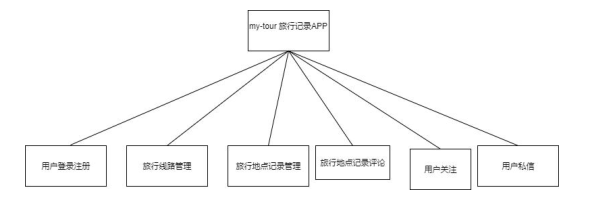
\includegraphics[width=0.7\textwidth]{system.png} %插入图片,[]中设置图片大小,{}中是图片文件名
    \caption{功能结构图} %最终文档中希望显示的图片标题
    \label{Fig.system} %用于文内引用的标签
  \end{figure}
\end{frame}

\begin{frame}{成果展示}
\end{frame}
\frame[plain, label=last]{
  \vspace{2.5cm}
  \hspace{1.7cm}
  \xiaoer  \begin{center} \textbf{\textit{Thanks for your attention! \\  \emptypar Q \& A }}\end{center}
  \vspace{2.5cm}
  \begin{flushright}
    \color{red}\it\xinwei\tiny 周翔辉\\[1.5pt]11603080122\\[1.5pt]软件工程\\[1.5pt]重庆理工大学两江
    人工智能学院
  \end{flushright}
} 

\end{document}
